\subsubsection*{A. A sad number} 

\problemauthor{ Абдикалыков А.К.}

Любое число $n$, начиная с 22, можно представить в виде суммы числа, начинающегося с двойки и числа, оканчивающегося двойкой: $n = 2\dots + \dots 2$. А среди чисел от 1 до 21 на требуемую сумму разбить можно только
числа 4 и 14.

Асимптотика: $O(1)$.



\subsubsection*{B. Brute force} 

\problemauthor{ Абдикалыков А.К.}

Рассмотрим $1 \leqslant a < b < \leqslant n$. Поскольку $(a, b) = \frac{b}{k}$ для некоторого натурального $k$, то $(a, b) \leqslant \frac{b}{2} \leqslant \left[ \frac{n}{2}\right]$. Значение в правой части достигается, если взять $a = \left[ \frac{n}{2}\right]$ и $b = 2 \left[ \frac{n}{2}\right]$.

Асимптотика: $O(1)$.

Замечание: прямой перебор $O(n)$ не проходит по ограничениям времени.



\subsubsection*{C. Curtains} 

\problemauthor{ Баев А.Ж.}

Вместо чисел $a_i$ будем хранить их разности $d_i = a_{i+1} - a_i$. Тогда запрос $a_i := a_i \pm 1$ будет
обрабатываться как: 
$$d_i: = di \mp 1, d_{i-1} := d_{i-1} \pm 1.$$ 

Чтобы быстро находить максимум, воспользуемся <<подсчетом>>: будем хранить $p_k$ --- сколько раз встречается число $k$ среди чисел $d_i$. Тогда увеличение $d_i$ на единицу влечёт следующие изменения:
$$p_{d_{i}} := p_{d_{i}}-1, p_{d_{i+1}} := p_{d_{i+1}} + 1.$$

Асимптотика: $O(N+Q)$.

Замечание: с помощью структур поиска (например, $multiset$) можно реализовать решение за $O(Q \log{N})$.



\subsubsection*{D. Dimitriy and broken sum} 

\problemauthor{ Абдикалыков А.К.}

Видно, что $a_i = i + b_i \dot 2^{k-1}$, где $b_i = \pm 1$. Значит,
$$ a_0 + a_1+ \dots + a_n = \frac{n(n + 1)}{2} + (b_0 + b_1 + \dots + b_n) \dot 2^{k-1}.$$

При этом суммы $b_i$ легко вычисляются --- это периодическая последовательность с периодом $2^k$, в начале которой идут $2^{k-1}$ единиц, затем $2^{k-1}$ минус единиц, и так далее.

Асимптотика: $O(1)$.



\subsubsection*{E. Excursion in snowy cube} 

\problemauthor{ Баев А.Ж.}

Рассмотрим взвещенный граф, в котором вершины --- это точки, а ребра --- это длина отрезка между точками в
пространстве.

Зафиксируем $L$. Далее построим кратчайший путь от вершины $A$ до вершины $B$ осуществляется с помощью алгоритма Дейкстры, при этом игнорируем все ребра весом более $L$. 

Очевидно, что если такой путь найдётся для
некоторого $L$, то он найдётся и для любого $L' > L$. Соответственно, подходящее $L$ можно найти бинарным поиском по $L$ из диапазона $[0; K]$ до соответствующей точности. При этом необходимо проверить существует ли вообще такое $L$ (если при $L = K$ такой путь не найдется, то ответ отрицательный).

Асимптотика: $O(N^2 \log{K})$.

Замечание: с помощью структур поиска можно реализовать быстрый алгоритм Дейкстры за $O(N \log{N} \log{K})$.



\subsubsection*{F. Food getting ways} 

\problemauthor{ Баев А.Ж.}

Пусть $u_i$ и $d_i$ --- число способов дойти
до верхнего и нижнего конца $i$-го переулка соответственно. Тогда ответом на задачу будет $d_n$, и его можно найти с помощью рекуррентных формул
$$
\begin{cases}
d_i := (d_{i-1} + u_{i-1}) \bmod M \\
u_i := u_{i-1}
\end{cases}
$$
если i-ый переулок вида {\tt ’/’} и
$$
\begin{cases}
d_i := d_{i-1}\\
u_i := (d_{i-1} + u_{i-1}) \bmod M
\end{cases}
$$
иначе.

Замечание: можно обойтись без хранения всего массивов $d$ и $u$, каждый раз обновляя только два текущих элемента.



\subsubsection*{G. Great and mighty} 

\problemauthor{ Баев А.Ж.}

Ответом являлось количество букв в записи числа
на трёх языках:
\begin{center}
\begin{tabular}{|c|c|c|}
\hline
десять & он & ten \\
\hline
6 & 2 & 3 \\
\hline
два & екi & two \\
\hline
3 & 3 & 3 \\
\hline
\end{tabular}
\end{center}



\subsubsection*{H. Hobby} 

\problemauthor{ Баев А.Ж.}

Определить, можно ли собрать замкнутую железную дорогу из $A$ прямых элементов и $B$ уголков. Очевидно, что оба числа в паре (A, B) должны быть чётными; также необходимо, чтобы уголков было как минимум 4 штуки. Рассмотрим сначала
случай $A \geqslant 2$. Нам понадобятся базовые сборки (2, 4) и (2, 6).

\begin{center}
\begin{minipage}{0.3\linewidth}
\begin{center}
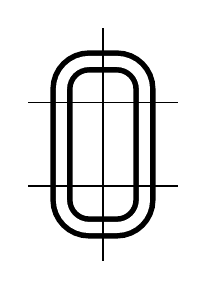
\begin{tikzpicture}[x=30,y=30]
\draw[rounded corners=10, line width=8pt] (0.5, 0.5) -- (0.5, 2.5) -- (1.5, 2.5) -- (1.5, 0.5) -- cycle;

\draw[color=white, rounded corners=10, line width=4pt] (0.5, 0.5) -- (0.5, 2.5) -- (1.5, 2.5) -- (1.5, 0.5) -- cycle;

\draw[step=1] (0.1, 0.1) grid (1.9, 2.9);
\end{tikzpicture}

$A = 2, B = 4$
\end{center}
\end{minipage}
\begin{minipage}{0.3\linewidth}
\begin{center}
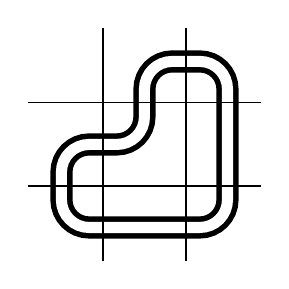
\begin{tikzpicture}[x=30,y=30]
\draw[rounded corners=10, line width=8pt] (0.5, 0.5) -- (0.5, 1.5) -- (1.5, 1.5) -- (1.5, 2.5) -- (2.5, 2.5) -- (2.5, 0.5) -- cycle;

\draw[color=white, rounded corners=10, line width=4pt] (0.5, 0.5) -- (0.5, 1.5) -- (1.5, 1.5) -- (1.5, 2.5) -- (2.5, 2.5) -- (2.5, 0.5) -- cycle;

\draw[step=1] (0.1, 0.1) grid (2.9, 2.9);
\end{tikzpicture}

$A = 2, B = 6$
\end{center}
\end{minipage}
\end{center}

%%%%%%%%%%%%%%%%%%%%%%%%

В любую уже построенную конструкцию можно добавить два прямых элемента. Соответственно, из конструкции с $(A, B)$ элементами, можно получить $(A+2, B)$.
\begin{center}
\begin{minipage}{0.3\linewidth}
\begin{center}
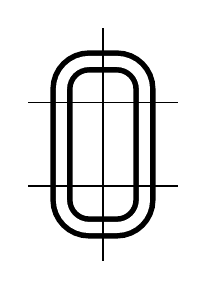
\begin{tikzpicture}[x=30,y=30]
\draw[rounded corners=10, line width=8pt] (0.5, 0.5) -- (0.5, 2.5) -- (1.5, 2.5) -- (1.5, 0.5) -- cycle;

\draw[color=white, rounded corners=10, line width=4pt] (0.5, 0.5) -- (0.5, 2.5) -- (1.5, 2.5) -- (1.5, 0.5) -- cycle;

\draw[step=1] (0.1, 0.1) grid (1.9, 2.9);
\end{tikzpicture}
\end{center}
\end{minipage}
\begin{minipage}{0.3\linewidth}
\begin{center}
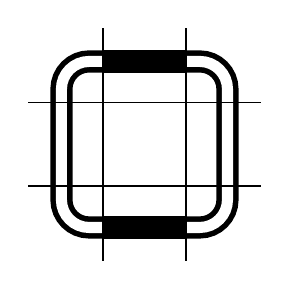
\begin{tikzpicture}[x=30,y=30]
\draw[rounded corners=10, line width=8pt] (0.5, 0.5) -- (0.5, 2.5) -- (2.5, 2.5) -- (2.5, 0.5) -- cycle;

\draw[color=white, rounded corners=10, line width=4pt] (0.5, 0.5) -- (0.5, 2.5) -- (2.5, 2.5) -- (2.5, 0.5) -- cycle;

\draw[line width=8pt] (1.0, 2.5) -- (2.0, 2.5);

\draw[line width=8pt] (1.0, 0.5) -- (2.0, 0.5);

\draw[step=1] (0.1, 0.1) grid (2.9, 2.9);
\end{tikzpicture}
\end{center}
\end{minipage}
\mbox{}

$(A, B) \rightarrow (A + 2, B)$
\end{center}

%%%%%%%%%%%%%%%%%%%%%%%%

Также в любую уже построенную конструкцию, где имеется хотя бы по два элемента каждого вида, можно добавить четыре уголка.

\begin{center}
\begin{minipage}{0.3\linewidth}
\begin{center}
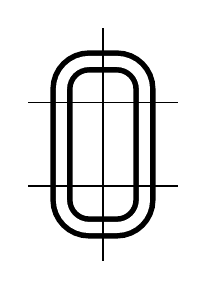
\begin{tikzpicture}[x=30,y=30]
\draw[rounded corners=10, line width=8pt] (0.5, 0.5) -- (0.5, 2.5) -- (1.5, 2.5) -- (1.5, 0.5) -- cycle;

\draw[color=white, rounded corners=10, line width=4pt] (0.5, 0.5) -- (0.5, 2.5) -- (1.5, 2.5) -- (1.5, 0.5) -- cycle;

\draw[step=1] (0.1, 0.1) grid (1.9, 2.9);
\end{tikzpicture}
\end{center}
\end{minipage}
\begin{minipage}{0.3\linewidth}
\begin{center}
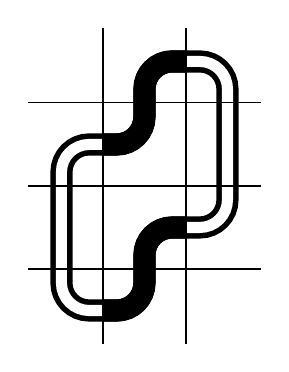
\begin{tikzpicture}[x=30,y=30]
\draw[rounded corners=10, line width=8pt] (0.5, 0.5) -- (0.5, 2.5) -- (1.5, 2.5) -- (1.5, 3.5) -- (2.5, 3.5) -- (2.5, 1.5) -- (1.5, 1.5) -- (1.5, 0.5) -- cycle;

\draw[color=white, rounded corners=10, line width=4pt] (0.5, 0.5) -- (0.5, 2.5) -- (1.5, 2.5) -- (1.5, 3.5) -- (2.5, 3.5) -- (2.5, 1.5) -- (1.5, 1.5) -- (1.5, 0.5) -- cycle;

\draw[rounded corners=10, line width=8pt] (1.0, 2.5) -- (1.5, 2.5) -- (1.5, 3.5) -- (2.0, 3.5);

\draw[rounded corners=10, line width=8pt] (2.0, 1.5) -- (1.5, 1.5) -- (1.5, 0.5) -- (1.0, 0.5);

\draw[step=1] (0.1, 0.1) grid (2.9, 3.9);
\end{tikzpicture}
\end{center}
\end{minipage}

$(A, B) \rightarrow (A, B + 4)$
\end{center}

Соответственно, можно построить дорогу для любой пары $(2n, 2m)$, где
$n > 1$, $m > 2$.

Рассмотрим отдельно $A = 0$. Несложно показать, что $B$ обязательно кратно четырем. Используя базовый пример $(0, 12)$ и перебрав меньшие варианты вручную, получаем, что возможны все конструкции вида $(0, 4k)$, кроме $(0, 8)$.



\subsubsection*{I. IMC problem} 

\problemauthor{ Абдикалыков А.К.}

Фиксируем число $k$. Посчитаем сколько чисел такого вида не превосходят $k$. Для это для каждой степени двойки такой, что $2^i \leqslant k$ достаточно перебрать все степени пятерки такой, что $5^j 2^i \leqslant k$. Ясно что итоговое количество таких чисел будет не больше, чем $\log_2{k} \log_5{k}$. Так количество подходящих чисел с ростом $k$ не уменьшается, то можно использовать бинарный поиск на отрезке $[0; 10^{18}]$.

Асимптотика: $O(\log^2{n})$.

Замечание: учитывая, что $n \leqslant 813$, можно просто сгенерировать все числа.



\subsubsection*{J. Join the knowledge} 

\problemauthor{ Абдикалыков А.К.}

Найдём число компонент связности обходом в ширину или глубину, и каждой клетке присвоим соответствующий номер. Если компонент больше 4, то ответ заведомо <<нет>>. В противном случае нужно будет перебрать все клетки со стенами и проверить, найдется ли среди них такая, которая имеет общую сторону с каждой компонентой связности.

Асимптотика: $O(n^2)$.



\subsubsection*{K. Keg and dipper} 

\problemauthor{ Баев А.Ж.}

Будем перебирать количество ковшей $N$ начиная с 1. Заметим, что ответ на задачу не меняется, если уменьшить все температуры на одно и тоже число. Уменьшим всё на $C$: $A_1 = A - C$, $B_1 = B - C$, $H_1 = H - C$. Остается найти такое $N$, что $A_1 \leqslant \frac{x H_1}{N} \leqslant B_1$. То есть существует целое $x$ между $\frac{A_1 N}{H_1}$ и $\frac{B_1 N}{H_1}$. Так как при $N = H_1$ данные числа будут гарантировано целыми, то перебор не превысит $H$ проверок.

Асимптотика: $O(H)$.



\subsubsection*{L. Lazy programming} 

\problemauthor{ Абдикалыков А.К.}

$\tau(k)$ является нечётным тогда и только тогда, когда $k$ --- точный квадрат. Таким образом, задача сводится к проверке на чётность число точных квадратов, не превосходящих $n$. Чётность искомой
суммы совпадает с чётностью числа $[\sqrt{n}]$.

Асимптотика: $O(1)$.